\documentclass{exam}
\usepackage{mainExam}

\title{Contrôle : Produit scalaire}
\date{2 Octobre 2024}
\author{Première Spécialité Mathématiques}

\begin{document}
\maketitle
\instructions{Interdite}

\begin{questions}
\vspace*{0.5cm}
\titledquestion{Plusieurs versions du produit scalaire}[5]
Pour chaque couple de vecteur $\vect{u}$ et $\vect{v}$ décris ci-après, donner le produit scalaire $\vect{u} \cdot \vect{v}$.
\begin{parts}
\part $\norm{\vect{u}} = \sqrt{2}$, $\norm{\vect{v}} = 2$ et $\cos(\widehat{\vect{u};\vect{v}}) = \dfrac{\sqrt{2}}{2}$.
\part $\norm{\vect{u}} = 7$, $\norm{\vect{v}} = 8$ et $\cos(\widehat{\vect{u};\vect{v}}) = -\dfrac{1}{2}$.
\part $\norm{\vect{u}} = 12^2$, $\norm{\vect{v}} = 13^3$ et $\widehat{\vect{u};\vect{v}} = 90°$
\part $\norm{\vect{u}} = 3$, $\norm{\vect{v}} = 4$ et $\norm{u-v} = 5$.
\part $\norm{\vect{u}} = 6$, $\norm{\vect{v}} = 6$ et $\norm{u+v} = 3$.
\end{parts}

\vspace*{0.5cm}
\titledquestion{Coordonnées de vecteurs}[4]
On se munit d'un repère orthonormé $(O,I,J)$.
\begin{center}
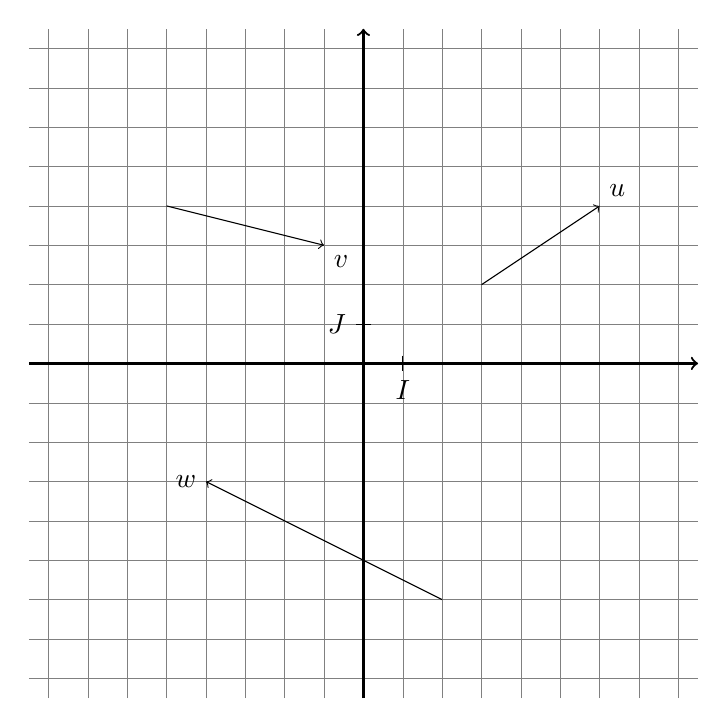
\begin{tikzpicture}
\draw[help lines] (-4.25,-4.25) grid[step=0.5] (4.25,4.25);
\draw[->,thick] (-4.25,0) -- (4.25,0);  
\draw[->,thick] (0,-4.25) -- (0,4.25);
\draw (0.1,0.5) -- (-0.1,0.5) node[left] {$J$};
\draw (0.5,0.1) -- (0.5,-0.1) node[below] {$I$};
\draw[->] (1.5,1) -- (3,2) node[above right] {$\vect{u}$}; 
\draw[->] (-2.5,2) -- (-0.5,1.5) node[below right] {$\vect{v}$};
\draw[->] (1,-3) -- (-2,-1.5) node[left] {$\vect{w}$};
\end{tikzpicture}
\end{center}
\begin{parts}
\part Donner les coordonnées des vecteurs $\vect{u}$, $\vect{v}$ et $\vect{w}$.
\part En déduire les produits scalaires $\vect{u} \cdot \vect{v}$, $\vect{u} \cdot \vect{w}$ et $\vect{v} \cdot \vect{w}$.
\part En déduire la valeur de $\vect{u} \cdot (\vect{v} + \vect{w})$.
\end{parts}
\newpage
\titledquestion{Démonstration}[4]
Soit $ABCD$ un carré. On pose un point $M$ mobile sur le segment $[BC]$, et on trace un triangle isocèle $BNM$ extérieur au carré $ABCD$. On note $b$ la longueur $BM$.
\begin{center}
\begin{tikzpicture}
\coordinate (A) at (0,0);
\coordinate (B) at (0,3);
\coordinate (C) at (3,3);
\coordinate (D) at (3,0);
\coordinate (M) at (1.5,3);
\coordinate (N) at (0,4.5);
\draw (A) node[below left] {$A$} 
    -- (B) node[left] {$B$}
    -- (C) node[above right] {$C$} 
    -- (D) node[below right] {$D$} 
-- cycle;
\draw (B) -- node[midway, sloped] {$|$} (N) node[above] {$N$} -- (M);
\draw (B) -- (M) node[midway] {$|$} node[below] {$M$};
\draw (B) ++(0,0.2) -- ++(0.2,0) -- ++(0,-0.2);
\end{tikzpicture}
\end{center}
\begin{parts}
\part En posant le repère orthonormé $(A;D;B)$, exprimer les coordonnées des points $A$, $M$, $N$ et $C$.
\part En déduire les coordonnées des vecteurs $\vect{AM}$ et $\vect{NC}$.
\part Calculer $\vect{AM} \cdot \vect{NC}$. Que peut-on en déduire pour les droites $(AM)$ et $(NC)$ ?
\end{parts}
\vspace*{0.5cm}
\titledquestion{Situation géométrique}[5]
Soit $ABCD$ un rectangle tel que $AB = 7$ et $AD = 3$. On pose $H$ le projeté orthogonal de $A$ par rapport à la droite $(DB)$ et $K$ le projeté orthogonal de $C$ par rapport à la droite $(DB)$. On cherche dans cet exercice la longueur $HK$
\begin{center}
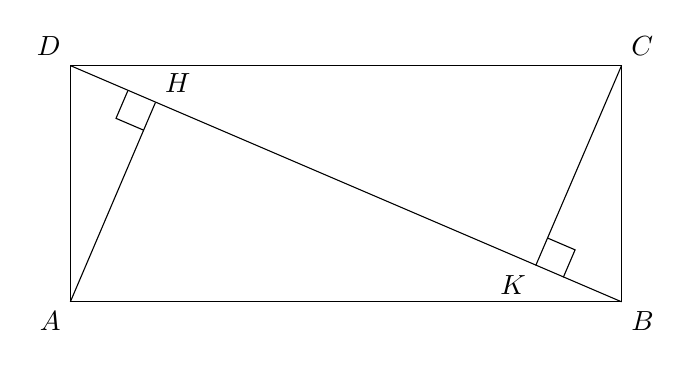
\begin{tikzpicture}
\coordinate (A) at (0,0);    
\coordinate (B) at (7,0);    
\coordinate (C) at (7,3);    
\coordinate (D) at (0,3);
\coordinate (H) at (1.08,2.53);
\coordinate (K) at (5.91,0.46);

\draw (A) node[below left] {$A$} 
    -- (B) node[below right] {$B$} 
    -- (C) node[above right] {$C$}
    -- (D) node[above left] {$D$}
-- cycle;
\draw (D) -- (B);
\draw (A) -- (H) node[above right] {$H$};
\draw (C) -- (K) node[below left] {$K$};

\draw (H) ++(-0.15,-0.35) -- ++(-0.35,0.15) -- ++(0.15,0.35);
\draw (K) ++(0.15,0.35) -- ++(0.35,-0.15) -- ++(-0.15,-0.35);

\end{tikzpicture}
\end{center}
\begin{parts}
\part Soient $\vect{u}$ et $\vect{v}$ deux vecteurs colinéaires. Rappeler la valeur de $\vect{u} \cdot \vect{v}$ en fonction de $\norm{\vect{u}}$, de $\norm{\vect{v}}$, et du sens des vecteurs $\vect{u}$ et $\vect{v}$.
\part En constatant que $\vect{AC} = \vect{AH} + \vect{HK} + \vect{KC}$, donner la valeur de $\vect{AC} \cdot \vect{DB}$ en fonction de $HK$ et de $DB$.
\part À l'aide de la projection orthogonale, donner les valeurs de $\vect{AC} \cdot \vect{AB}$ et de $\vect{AC} \cdot \vect{AD}$.
\part En remarquant que $\vect{DB} = \vect{DC} + \vect{CB}$, et à l'aide de la question précédente, calculer d'une nouvelle manière $\vect{AC} \cdot \vect{DB}$.
\part Conclure en donnant la valeur exacte de $HK$ à l'aide des questions précédentes. 
\end{parts}
\vspace*{0.5cm}

\end{questions}
\end{document}